\documentclass[border=4pt]{standalone}
\usepackage[T1]{fontenc}
\usepackage{lmodern}
\usepackage{pgfplots}

\pgfplotsset{compat=1.18}
\definecolor{editblue}{HTML}{193E57}
\definecolor{lawgray}{HTML}{81888C}

\begin{document}
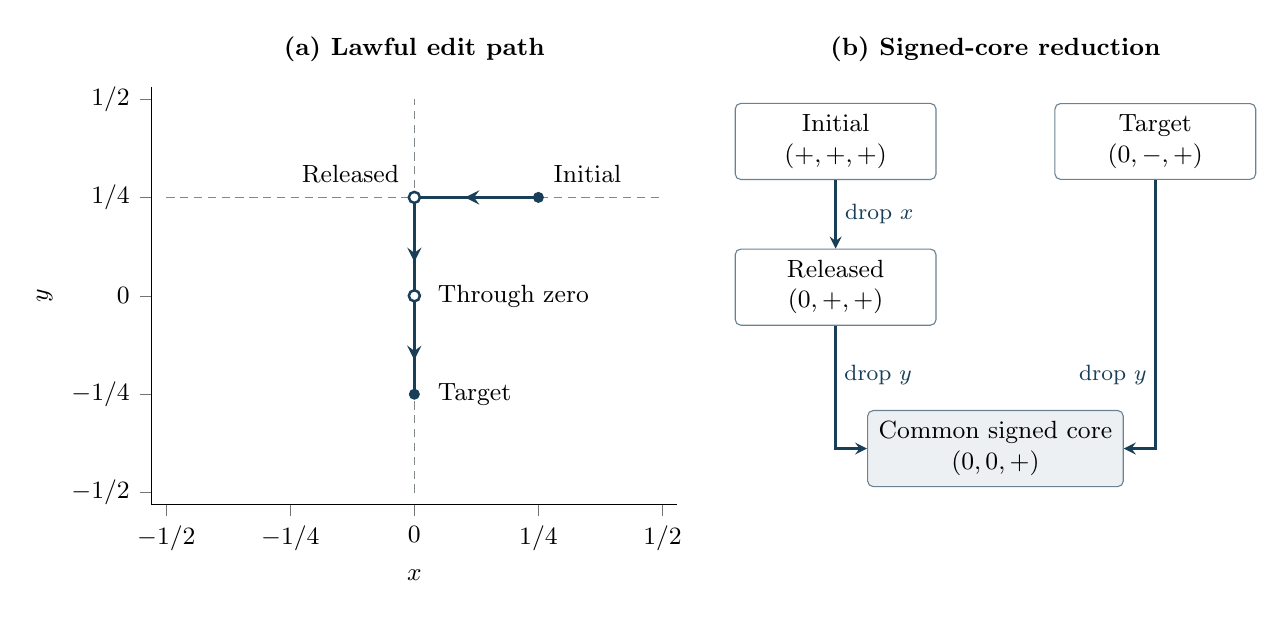
\begin{tikzpicture}
\begin{axis}[
  width=6.68cm,
  height=5.30cm,
  scale only axis,
  anchor=south west,
  xmin=-0.53, xmax=0.53,
  ymin=-0.53, ymax=0.53,
  axis lines=left,
  axis line style={-},
  tick align=outside,
  tick style={black!55},
  ticklabel style={font=\small},
  xlabel={$x$},
  ylabel={$y$},
  label style={font=\small},
  xtick={-0.5,-0.25,0,0.25,0.5},
  ytick={-0.5,-0.25,0,0.25,0.5},
  xticklabels={$-1/2$,$-1/4$,$0$,$1/4$,$1/2$},
  yticklabels={$-1/2$,$-1/4$,$0$,$1/4$,$1/2$}
]
\addplot[lawgray,thin,densely dashed] coordinates {(-0.5,0.25) (0.5,0.25)};
\addplot[lawgray,thin,densely dashed] coordinates {(0,-0.5) (0,0.5)};

\draw[editblue,line width=1.25pt]
  (axis cs:0.25,0.25) -- (axis cs:0,0.25) -- (axis cs:0,-0.25);
\draw[editblue,line width=1.25pt,-stealth]
  (axis cs:0.176,0.25) -- (axis cs:0.102,0.25);
\draw[editblue,line width=1.25pt,-stealth]
  (axis cs:0,0.16) -- (axis cs:0,0.086);
\draw[editblue,line width=1.25pt,-stealth]
  (axis cs:0,-0.090) -- (axis cs:0,-0.163);

\fill[editblue] (axis cs:0.25,0.25) circle (2pt);
\fill[editblue] (axis cs:0,-0.25) circle (2pt);
\filldraw[fill=white,draw=editblue,line width=0.9pt]
  (axis cs:0,0.25) circle (2pt)
  (axis cs:0,0) circle (2pt);

\node[font=\small,anchor=south west,xshift=2pt,yshift=2pt]
  at (axis cs:0.25,0.25) {Initial};
\node[font=\small,anchor=south east,xshift=-2pt,yshift=2pt]
  at (axis cs:0,0.25) {Released};
\node[font=\small,anchor=west,xshift=5pt]
  at (axis cs:0,0) {Through zero};
\node[font=\small,anchor=west,xshift=5pt]
  at (axis cs:0,-0.25) {Target};
\end{axis}

\node[font=\small\bfseries] at (3.34,5.78) {(a) Lawful edit path};

\begin{scope}[
  shift={(7.30cm,0cm)},
  state/.style={
    draw=editblue!65, rounded corners=2pt, inner sep=4pt,
    minimum width=2.55cm, minimum height=9mm, align=center, font=\small
  },
  contraction/.style={editblue,line width=0.9pt,-stealth},
  step label/.style={font=\footnotesize,inner sep=3pt,text=editblue}
]
\node[font=\small\bfseries] at (3.42,5.78) {(b) Signed-core reduction};

\node[state] (initial) at (1.39,4.61) {Initial\\$(+,+,+)$};
\node[state] (target) at (5.45,4.61) {Target\\$(0,-,+)$};
\node[state] (released) at (1.39,2.76) {Released\\$(0,+,+)$};
\node[state,fill=editblue!8,minimum width=3.13cm] (core) at (3.42,0.71)
  {Common signed core\\$(0,0,+)$};

\draw[contraction] (initial.south) --
  node[step label,right] {drop \(x\)} (released.north);
\draw[contraction] (released.south) |- (core.west);
\draw[contraction] (target.south) |- (core.east);
\coordinate (second label row) at (0,1.65);
\node[step label,right] at (released.south |- second label row) {drop \(y\)};
\node[step label,left] at (target.south |- second label row) {drop \(y\)};
\end{scope}

\end{tikzpicture}
\end{document}
